{\bf Суперкомпиляция} --- метод анализа и преобразования программ,
который отслеживает обобщённую возможную историю вычислений исходной программы и строит
на её основе эквивалентную ему программу, структура которой, в некотором смысле, ``проще''
структуры исходной программы\cite{turchinSC}. % Турчин

Это упрощение достигаются путём удаления или преобразования
некоторых избыточных действий: удаление лишнего кода, выполнение операций над
уже известными данными, избавление от промежуточных структур данных, инлайнинг и т.п.

Суперкомпиляция включает в себя частичные вычисления, однако не сводится к ним полностью
и может привести в глубоким структурным изменениям оригинальной программы.

Суперкомпиляторы, которые используют только ``положительную'' информацию
--- то есть информацию о том, что сводобные переменные чему-то равны, ---
называют позитивными~\origin{positive supercompilation}\cite{scPos}.
К примеру, при достижении условного выражения {\bf if} x $=$ a {\bf then} $t_1$ {\bf else} $t_2$
позитивный суперкомпилятор при вычислении $t_1$ будет учитывать то, что x $=$ a,
однако при вычислении $t_2$ он не будет знать, что x $\neq$ a.
Расширение позитивного компилятора c поддержкой такой ``негативной'' информации --- идеальный
суперкомпилятор~\origin{perfect supercompilation}\cite{scPerf}.

% Про "символьное исполнение" https://en.wikipedia.org/wiki/Symbolic_execution
% Сделать ссылку на Ключникова?
%История вычислений представляется в виде {\it графа конфигураций}, где {\it конфигурация}
%описывает состояние вычисления на конкретном шаге. Построение графа происходит на этапе
%{\it прогонки}, во время которого происходит символьное исполнение программы. Потенциально
%такой граф --- который без дополнительных шагов прогонки вырождается в дерево ---
%бесконечный. Для трансформации бесконечного дерева в конечный объект используется {\it cвёртка}
%--- при обработке конфигурации, выражение в которой является {\it переименованием} выражения в одной
%из родительских конфигураций.

История вычислений представляется в виде \emph{графа процессов} --- корневого ориентированного графа,
в котором каждая ветвь --- это отдельный путь вычислений, а каждый узел --- состояние системы или \emph{конфигурация}.
Конфигурация обобщённо описывает множество состояний вычислительной системы или её подсистемы.
% К примеру, конфигурацией можно назвать пару из выражения $1 + x$, которое описывает все возможные суммы с $1$
% свободной переменной $x$, и множество органичений $\{ x \neq 10, x = 1 + x_1 \}$,
% которое сужает множество описываемых состояний до необходимого.
К примеру, конфигурацией можно назвать выражение $1 + x$, в котором параметр $x$ пробегает
все возможные значения своего домена (допустим, множество натуральных чисел) и задаёт
таким образом множество состояний программы. 

Процесс построение графа процессов называется \emph{прогонкой}~\origin{driving}.
Во время прогонки производится шаг символьных вычислений, после которого
в граф процессов добавляются порождённые конфигурации; множество конфигураций
появляются тогда, когда ветвления в программе зависят от свободных переменных.

В процессе прогонки в конфигурациях могут появляться новые свободные переменные,
которые строятся из исходной конфигурации:
если при вычислении выражение его переменная перешла в другую переменную (к примеру, из-за сопоставления с образцом),
то в итоговую конфигурацию будет подставлена новая переменная и связь старой и новой сохранится в
некоторой \emph{подстановке}.
Подстановка --- это отображение из множества переменных в множество возможно замкнутых термов.
Применение подстановки к выражению заменит все вхождения переменных, принадлежащих её домену,
на соответствующие термы. \todo{Что-нибудь ещё}

Пример графа процессов представлен на рисунке~\ref{fig:pgraphExample}.

\begin{figure}[h!]
\center
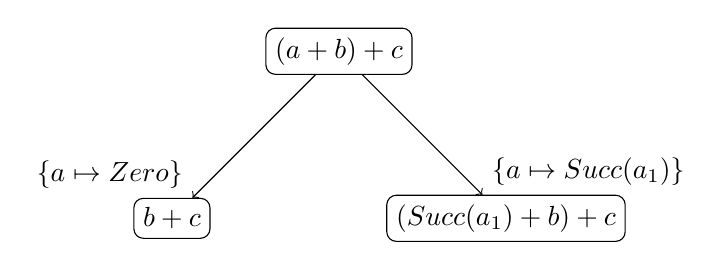
\begin{tikzpicture}[->,node distance=3cm, sibling distance=5cm]
                                                            
  \tikzstyle{conf}=[rectangle,draw, rounded corners=.8ex]

  \node[conf] (root) {$(a + b) + c$} ;
  \node[conf] (childLeft) [below left of = root] {$b + c$};
  \node[conf] (childRight)[below right of = root] {$(\text{Succ}(a_1) + b) + c$};
  \path (root) edge node[above left,pos=1] {$\{a \mapsto \text{Zero}\}$} (childLeft)
        (root) edge node[above right,pos=1]{$\{a \mapsto \text{Succ}(a_1)\}$}(childRight);
\end{tikzpicture}

\label{fig:pgraphExample}
\caption{Пример части графа процессов.}
\end{figure}

Потенциально процесс прогонки бесконечный, к примеру, когда происходят рекурсивные вызовы.
Для превращения бесконечого дерева вычисления в конечный объект, по которому множно
восстановить исходное дерево, используется \emph{свёртка.}

Свёртка~\origin{folding}~--- это процесс преобразования дерева процессов в граф, при котором
из вершины $v_c$ добавляется ребро в родительскую вершину $v_p$,
если выражение в конфигурации в $v_c$ и в $v_p$ равны с точностью до переименования.
Пример ситуации для свёртки изображён на рисунке~\ref{fig:pgraphFoldingExample},
на котором свёрточное ребро изображено пунтктиром.

\begin{figure}[h!]
\center
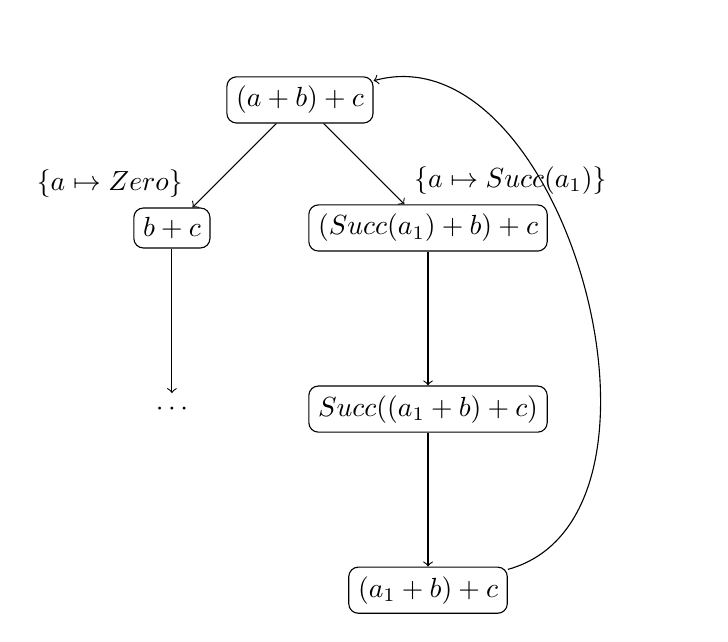
\begin{tikzpicture}[->,node distance=2.3cm, sibling distance=5cm]
                                                            
  \tikzstyle{conf}=[rectangle,draw, rounded corners=.8ex]

  \node[conf] (root) {$(a + b) + c$} ;
  \node[conf] (childLeft) [below left of = root] {$b + c$};
  \node[conf] (childRight)[below right of = root] {$(\text{Succ}(a_1) + b) + c$};
  \node[conf] (childRight2)[below  of = childRight] {$\text{Succ}((a_1 + b) + c)$};
  \node[conf] (childRight3)[below  of = childRight2] {$(a_1 + b) + c$};
  \node (left)[below of = childLeft] {$\cdots$};

  \path (root) edge node[above left,pos=1] {$\{a \mapsto \text{Zero}\}$} (childLeft)
        (root) edge node[above right,pos=1]{$\{a \mapsto \text{Succ}(a_1)\}$}(childRight)
        (childLeft) edge (left)
        (childRight) edge (childRight2)
        (childRight2) edge (childRight3)
        (childRight3) edge[bend right=90] (root);
\end{tikzpicture}

\label{fig:pgraphFoldingExample}
\caption{Пример свёртки.}
\end{figure}

Однако существует ситуации, при котором свёртка не привёт к тому, что граф превратится в
конечный объект. Такое может произойти, к примеру, когда два выражения структурно
схожи, но не существует переименования, уравнивающих их: $a + b$ и $a + a$.

Для решения этой проблемы используется \emph{обобщение}\cite{scGen}. Обобщение --- это процесс
замены одной конфигурации на другую, более абстрактную, описывающую больше состояний
программы. Для обнаружения ``похожей'' конфигурации используется предикат,
традиционно называемый \emph{свистком}. Сам шаг обобщения может произвести дейтсвия трёх видов:
\begin{itemize}
\item \emph{обобщение вниз} приводит к тому, что новая конфигурация заменяет текущую в графе процессов;
\item \emph{обобщение вверх} приводит к замене родительской конфигурации на обобщённую;
\item \emph{разделение}~\origin{split} используется для декомпозиции выражений, которые затем
будут обработаны отдельно.
\end{itemize}

\todo{вроде надо бы что-нибудь ещё написать про это вот всё}
